\documentclass[12pt,letterpaper,noanswers]{exam}
\usepackage[usenames,dvipsnames,svgnames,table]{xcolor}
\usepackage[margin=0.9in]{geometry}
\renewcommand{\familydefault}{\sfdefault}
\usepackage{multicol}
\usepackage{wrapfig}
\pagestyle{head}
\definecolor{c03}{HTML}{FFDDDD}
\header{AM 22b Class 01}{}{Jan 25: Activity + Intro}
\runningheadrule
\headrule
\usepackage{graphicx} % more modern
\usepackage{amsmath} 
\usepackage{amssymb} 
\usepackage{hyperref}
\usepackage{tcolorbox}

\usepackage[numbered,autolinebreaks,useliterate]{mcode}


\begin{document}
 \pdfpageheight 11in 
  \pdfpagewidth 8.5in
\vspace{0.5cm}

%\noindent Name:\rule{3in}{1pt}

%\noindent\textbf{Activity}

\noindent What is the flow of the Charles River near the location of the Weeks footbridge?


\noindent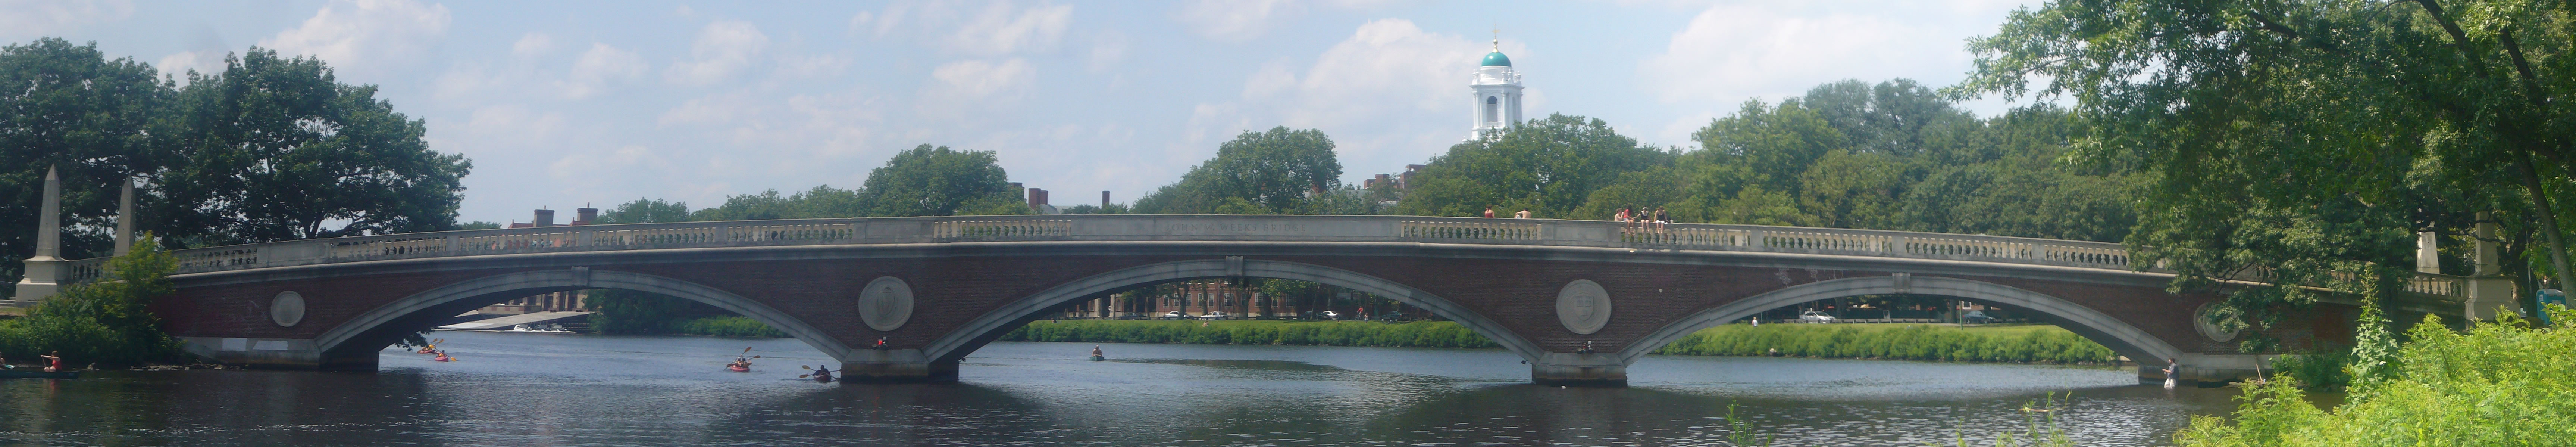
\includegraphics[width=\textwidth]{img/Weeks_footbridge_panorama.jpg}



\noindent photo by Austin Donisan, CC BY 3.0, \url{https://commons.wikimedia.org/w/index.php?curid=7387981}

\begin{enumerate}
\item What do you think I mean by `flow'?

\emph{Think about this, and type your thoughts into the Zoom chat.  Don't press `enter' until you're asked to: we'll all submit our ideas at the same time}

\item Open the Jamboard for today.  The link is available on the front page of our course Canvas site.
\begin{itemize}
\itemsep0em
    \item In Jamboard, find you assigned slide/frame/page (page numbers are assigned below).  
    \item Write or type your name in the corner of your slide.
    \item Consider question 3 (below) and make notes or write your thoughts on your Jamboard slide.
\end{itemize}

\begin{multicols}{4}
1. student names here.
\end{multicols}

\item Think about how you might measure or approximate the flow of the Charles River near the footbridge.  As part of your thinking, consider what information (data) would be helpful.

\emph{Make notes or sketches on your Jamboard slide}.



\item Within zoom, move to the breakout room that corresponds to your assigned group.

\begin{multicols}{3}
1. student names here
\end{multicols}

Introduce yourself to the people in your group.  Discuss your ideas from question 3 together.  Use screen sharing to look at each other's notes/slides.

\item Choose one of your slides and add the names of the other members of the team.  Work together to choose a method for approximating the flow.  Make sure to include the following information:

\begin{itemize}
\item Data you would need:
\item Procedure for approximating the flow using the data:
\item Dimensions of the output of your procedure (mass ($M$)? length ($L$)? time ($T$)? $L^2$? $L/T$? etc):
\end{itemize}
\end{enumerate}

\eject

% \noindent\textbf{Survey}

% \begin{enumerate}
% \item Did you take APMTH 22a last semester?  Yes\rule{0.5in}{1pt}\quad No\rule{0.5in}{1pt}
    
% \item What mathematics course did you take prior to taking APMTH 22a?
% \vspace{1in}
    
% \item Concentration or intended concentration:
% \vspace{0.4cm}

% \item Write briefly based on the following:  ``I feel supported in my learning when...''
% \vspace{3cm}
% \end{enumerate}

\eject


% I need to review the torus trajectories...

\begin{itemize}
\itemsep0em
    %\item The first skill check will be in class on Friday.  There will be a sample problem on Wednesday.
    \item There will be a pre-class assignment (assigned Friday after class) for Monday Feb 1st.  It will be made available via Canvas.
    \item The first problem set and first WeBWorK assignment will be assigned at the end of this week and will be due Thursday Feb 6th.
    \item Office hour information is posted on the Canvas site.  Sarah has office hours today at 3pm if you have questions about the course.
    \item Use the link on Canvas to Slack to join our course Slack channel before Wednesday's class meeting.  Within Slack I have enabled free-response anonymous polls, which we will occassionally use during class.
\end{itemize}

\hrule
\vspace{0.2cm}



\noindent\textbf{Big picture}

As a preview to some of the ideas in the course, we will begin with an activity that introduces a concept from later in the semester.  I will also share information about the course, including its structure and content.

\vspace{0.2cm}

\hrule
\vspace{0.2cm}

\noindent\textbf{River flow activity}


\vspace{0.2cm}
\hrule
\vspace{0.2cm}


\noindent\textbf{Activity vocabulary}
\begin{tcolorbox}
The \textbf{flux} of water in a river is the rate at which a volume of water is crossing a cross-section of the river.  The dimensions are $L^3/T$ (length cubed over time).

In this context a \textbf{cross-section} is an imaginary surface that cuts across the river.  

A \textbf{surface} is a two-dimensional manifold. \url{https://en.wikipedia.org/wiki/Surface#In_mathematics}

For the purposes of this course, a \textbf{manifold} is a space that looks like Euclidean space when you zoom in.  Examples: A line is a 1d Euclidean space.  A circle (the boundary curve of a disk) is a 1d manifold.  A plane is a 2d Euclidean space.  A sphere (the boundary of a ball) is a 2d manifold.

\end{tcolorbox}

\noindent\textbf{River flow data}

The image below shows measured velocities along a cross-section of a river (the confluence of the White River and the Wabash River near the Illinois-Indiana border).  The water from the White River is on the left and from the Wabash is on the right: you may be able to see (from the white arrows) that they are still behaving a bit like two separate streams of water.

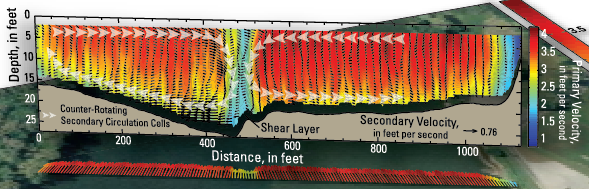
\includegraphics[width=\textwidth]{img/C01adcpUSGS-2.png}

\url{https://hydroacoustics.usgs.gov/movingboat/VMT/VMT_Example2.png}

\url{https://hydroacoustics.usgs.gov/movingboat/VMT/VMT.shtml}

\begin{itemize}
\setlength{\itemsep}{0em}
    \item The shape of the river cross-section is visible.
    \item The velocity downstream is shown using color.
    \item The lateral velocity (water motion within the cross-section) is shown using short arrows.
    \item At each point in the cross-section, the water has an associated velocity vector in 3-space.  That velocity vector has been decomposed into a component parallel to the cross-section (lateral) and one perpendicular to the cross-section (downstream).
\end{itemize}

\noindent\textbf{Approximating the flux}

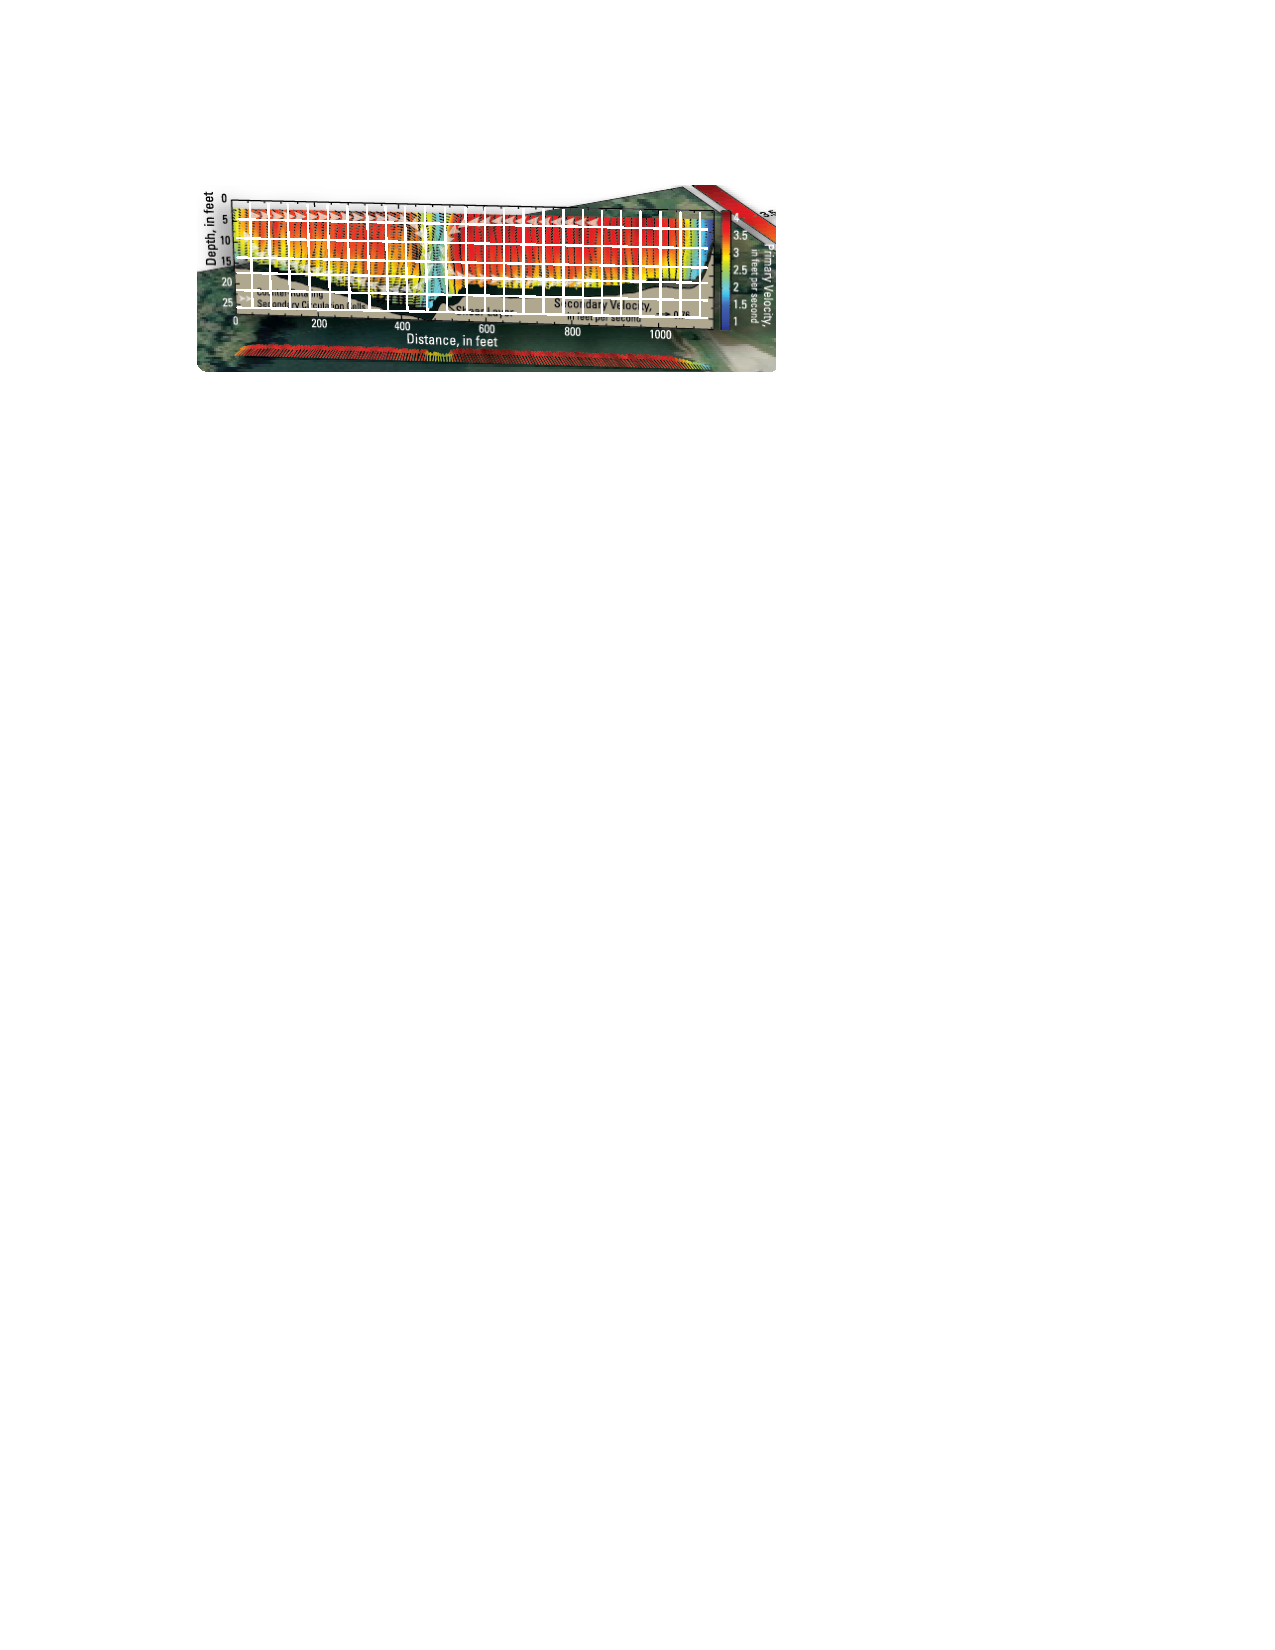
\includegraphics{img/C01adcpUSGS-3.pdf}

Here's one method for approximating the flux.
\begin{itemize}
\itemsep0em
    \item Divide the region into small squares.
    \item Identify the area of river cross-section, $A_k$, that exists within each square $k$.
    \item For each square, compute a representative downstream water speed measurement, $s_k$.  One way to do this is by averaging all of the measurements taken within the square.  Another way to do this is by selecting a single measurement at random from within the square.
    \item Compute an approximation of the flux through the $k$th square by multiplying the area of the square and the water speed: $A_k*s_k$.
    \item Sum the approximate flux through each small square, $\sum_{k\in \# \text{squares}} A_ks_k$, to find an approximate total flux.
\end{itemize}

\noindent\textbf{Finding the exact flux}

If we had a function giving us the velocity of the river at each point in the cross section:
\begin{itemize}
\itemsep0em
    \item We would compute the component of the velocity pointing perpendicular to the cross section to find a function for $s$, the downstream water speed.
    \item We would treat our sum above as a Riemann sum.  We would take the limit as the area of the boxes goes to zero to turn the sum into an integral.
    \item We would then integrate over the region to find the flux.
\end{itemize}

We will learn to set up integrals over regions in a few weeks.  We will learn to compute surface integrals and flux integrals in late March or early April.

% \noindent \textbf{Vocabulary}
% \begin{tcolorbox}
% \begin{multicols}{4}
% \begin{enumerate}
% \setlength\itemsep{-0.5em}
%     \item function
%     \item graph
%     \item expression
%     \item equation
%     \columnbreak
%     \item linear
%     \item differential equation
%     \item variable
%     \item constant
%     \item parameter
%     \item independent variable
%     \item dependent variable
%     \item vector
%     \item scalar
%     \item vector function
%     \item scalar function
%     \item contour
% \end{enumerate}
% 
% \end{multicols}
% \end{tcolorbox}

\vspace{0.2cm}
\hrule
\vspace{0.2cm}

\noindent\textbf{Course information interlude}

\vspace{0.2cm}
\hrule
\vspace{0.2cm}
\noindent\textbf{Coordinate axes in 3-space}

\begin{tcolorbox}
A \textbf{right-handed coordinate system} is a 3d coordinate system in which the axes satisfy the right-hand rule.  \url{http://mathworld.wolfram.com/Right-HandedCoordinateSystem.html}

The \textbf{right hand rule} is a convention for setting axis labels and vector directions.  Under this convention, in a right-handed coordinate system $a_1a_2a_3$, if you point your right index finger along the first axis direction, $a_1$, and your right second finger (pointer finger) along the second axis direction, $a_2$, your right thumb can easily be pointed along the third axis direction $a_3$.

A \textbf{left-handed coordinate system} would use a left-hand rule.  By convention, we will not use left-handed coordinate systems this semester.
\end{tcolorbox}

\vspace{0.2cm}

\hrule
\vspace{0.2cm}
\noindent\textbf{Poll}

\eject
% \noindent\textbf{Matlab code example 1}
% \begin{lstlisting}
% %% Class 01.  Example 01.
% % Plot a curve in 2-space (in the xy-plane).
% syms x
% f = @(x) sin(x*pi/30);
% fplot(x,f(x),[0,30],'LineWidth',3)
% xlabel('x'); ylabel('y')
% title('curve: y = sin(\pi x/30)')
% set(gca,'FontSize',10)
% % Choose an axis range.
% axis equal; axis([0 30 -2 2])
% % I adjusted the size of the figure by hand before saving.
% print('-opengl','~/Desktop/sinewave.eps','-depsc','-r300')
% \end{lstlisting}

% \includegraphics[width=\textwidth]{img/sinewave.eps}

% \vspace{0.2cm}
% \hrule
% \vspace{0.2cm}

% \noindent\textbf{Matlab code example 2}
% \begin{lstlisting}
% %% Class 01.  Example 02.
% xvals = 0:1:30;
% fvals = sin(xvals*pi/30);
% plot(xvals,fvals,'-*','LineWidth',3)

% % This makes a similar plot.
% % It doesn't use the symbolic toolbox.
% % It is plotting points (xk,yk) for
% % x = 0,1,2,...,30 and
% % y = f(0), f(1),...,f(30).

% xlabel('x'); ylabel('y')
% title('curve: y = sin(\pi x/30)')
% set(gca,'FontSize',10)
% axis equal
% axis([0 30 -2 2])
% print('-opengl','~/Desktop/sinewave2.eps','-depsc','-r300')
% \end{lstlisting}

% \includegraphics[width=\textwidth]{img/sinewave2.eps}

\end{document}